%%%% SEITENRAENDER, SCHRIFTGROESSE UND ZEILENABSTAND NICHT ABAENDERN => SONST GIBT ES PUNKTEABZUG
\documentclass[a4paper,11pt,singlespacing]{article}
% \usepackage[left=2.5cm,right=2.5cm,top=2.5cm]{geometry}
\usepackage{setspace}
\usepackage[utf8]{inputenc}
\usepackage[T1]{fontenc}
\usepackage{graphicx}
\usepackage[ngerman]{babel}
\usepackage{color}
\usepackage{wrapfig}
\usepackage{titleref}
\usepackage{hyperref}
\usepackage[rightcaption]{sidecap}
\usepackage{listings,xcolor}
\usepackage[numbers,round]{natbib}
\usepackage{textcomp}
\usepackage{float} % For image floating ([H] -> "here")

% Configuration
\sloppy
\graphicspath{ {images/} }

% Cover setup
\title{Systemadministration - Mailserver Honeypot zum analysieren von Spam}
\author{Manuel Adams 27470, Michael Ruf 27428, Mario Waizenegger 29608}

\begin{document}
\setlength{\parindent}{0ex} % Absatzeinrückung verhindern
\pagenumbering{roman}

\maketitle

\begin{abstract}
Heutzutage wird viel \nameref{itm:Spam} verschickt. Einiges davon wird erkannt und gefiltert.
Um die Analyse von Spam-Nachrichten und deren Versender zu ermöglichen, wird ein Mailserver \nameref{itm:Honeypot} aufgesetzt.
Dieser soll \nameref{itm:Spam}-Nachrichten erhalten können, sowie als offener Verteiler für Spammer verfügbar sein.
\end{abstract}

\newpage

% Table of contents
\tableofcontents

\newpage
\pagenumbering{arabic}

% Content
\section{Einleitung}\label{sec:Einleitung}
	% NOTE "Wir" erlaubt
	Warum \nameref{itm:Spam} versandt wird ist vielen Menschen ein Rätsel.
	Das wirft die Fragen auf, wer Spam versendet und was die Beweggründe von Spammern sind.
	Wie geht man mit Spam um und was passiert wenn man auf \nameref{itm:Spam} reagiert?
	Ein \nameref{itm:Spam} \nameref{itm:Honeypot} bietet die Möglichkeit diese Fragen zu analysieren und die nötigen Daten zu erheben.
	% NOTE Warum lohnt sich das?
	\\
	Da die Methoden von erfolgreichen Spammern nicht dokumentiert sind, ist das Bekanntmachen des "`\nameref{itm:OpenRelay}"'"~Servers schwierig.
	Zudem ist es zeitaufwendig die eigenen Mail-Adressen unter Spammern bekannt zu machen und viele authentische Spam-Mails in kurzer Zeit zu erhalten eine Herausforderung.
	% NOTE Man kann man beim Ergebnis nochmal Stellungnahme hierzu nehmen oder den Text hier ergänzen
	% -----
	% - Wirtschaftlichkeit
	% - Andere Beweggründe
	% - Findet man Informationen über Systeme, von denen Spam verschickt wird?
	% - Werden die Nachrichten generiert? (Bots)

	\subsection{Ziel der Arbeit}\label{sec:EinleitungZiel}
		Es soll durch einen Mailserver Honeypot Erkenntnisse über Herkunft, Zweck und Zielgruppe von \nameref{itm:Spam} Nachrichten erhalten werden.
		Zusätzlich soll erarbeitet werden welche weiteren nützlichen Informationen man den Mails entnehmen kann.
		Durch diese Informationen soll die Motivation von Spammern besser verstanden und entsprechende Vorkehrungen zum Schutz ermöglicht werden.
		% NOTE Was wird genau analysiert
	
	\subsection{Vorgehensweise}\label{sec:EinleitungVorgehensweise}
		Um den Honeypot zu realisieren muss der Mail-Dienst aus dem Internet zugänglich sein.
		Dieser besteht hierbei aus Ausgangsserver und Eingangsserver.
		Hierzu werden auf einer \nameref{itm:VirtuelleMaschine} die Dienste in \nameref{itm:Container}n aufgesetzt.
		Aus Sicherheitsgründen muss die VM ins interne Netz abgeschottet sein.
		Der Aufbau ist in \autoref{fig:Hierarchy} visualisiert.

		\begin{figure}[H]
		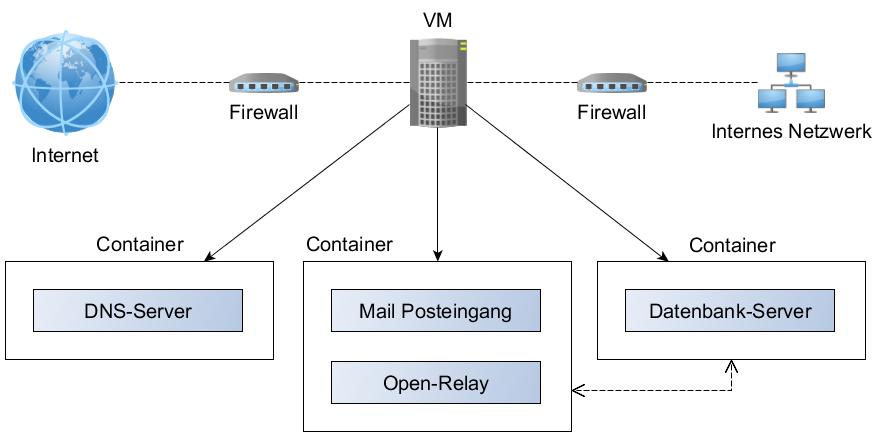
\includegraphics[width=\linewidth]{2-Hierarchy.png}
		\caption{Netzwerkstruktur}
		\label{fig:Hierarchy}
		\end{figure}

		Um den Eingangsserver zu realisieren sind folgende Aufgaben erforderlich:
		\begin{enumerate}
		\item Mail Eingangsserver bereitstellen und konfigurieren
		\item \nameref{itm:DNS} Server einrichten um realistische E-Mail-Adressen bereitzustellen
		\item Bei möglichst vielen Diensten mit unterschiedlichen Mailadressen registrieren
		\item Mails analysieren indem per Script geprüft wird, ob sich Informationen  über den Versender ermitteln lassen.
		\end{enumerate}

		Den Ausgangsserver betreffend sind folgende Aufgaben erforderlich:
		\begin{enumerate}
		\item Mail Ausgangsserver bereitstellen und konfigurieren
		\item Als "`\nameref{itm:OpenRelay}"' im Internet durchsickern lassen
		\item Eingehende Mails tatsächlich weiterleiten
		\item Mails analysieren
		\end{enumerate}

	\subsection{Aufbau der Arbeit}\label{sec:EinleitungAufbau}
		\begin{itemize}
			\item
				In Abschnitt 1 werden die nötigen Grundbegriffe zum Verständnis abgesteckt.
			\item
				In Abschnitt 2 wird das Projekt und die Zielsetzung zusammengefasst.
			\item
				In Abschnitt 3 geht es die Problemstellung des Projekts.
			\item
				In Abschnitt 4 werden die zu erarbeitenden Ziele genannt.
			\item
				In Abschnitt 5 werden mögliche technische Lösungen zur Problemstellung benannt und bewertet.
			\item
				In Abschnitt 6 werden die am besten passenden Lösungen aus Abschnitt 5 genannt.
			\item
				In Abschnitt 7 wird beschrieben wie die tatsächliche Umsetzung anhand der technischen Lösungen aus Abschnitt 6 aussieht.
			\item
				In Abschnitt 8 wird das Projekt nochmals zusammengefasst und ein Fazit gezogen.
		\end{itemize}

\newpage

\section{Grundbegriffe}\label{sec:Grundbegriffe}
	Die folgenden Begriffsdefinitionen und Unterscheidungen sind zum einen zur Verdeutlichung, wie Begriffe in dieser Arbeit verstanden werden und um Fachbegriffe zu erklären.
	
	% NOTE Alle nochmal durchnudeln
	\begin{description}
	\item[Spam\label{itm:Spam}]\hfill \\
		Als Spam oder Junk werden unerwünschte, in der Regel auf elektronischem Weg übertragene Nachrichten[...] bezeichnet, die dem Empfänger unverlangt zugestellt werden und häufig werbenden Inhalt enthalten. Dieser Vorgang wird Spamming oder Spammen genannt, der Verursacher Spammer.\cite{Spam}
	\item[Honeypot\label{itm:Honeypot}]\hfill \\
		Sicherheitstechnisch scheinbar verwundbares Computerprogramm, das Computerviren, -würmer und Trojaner anlockt, um sie zu registrieren und unschädlich zu machen.\cite{Honeypot}
	\item[Open-Relay\label{itm:OpenRelay}]\hfill \\
		Ein SMTP-Relay-Server der durch unzureichende Sicherheitskonfiguration auch Mails weiterleitet bei denen er weder für die Absender- noch für die Zieladresse zuständig ist, wird als "`Open relay"' bezeichnet.\cite{SMTP-Relay-Server}
	\item[Virtuelle Maschine (VM)\label{itm:VirtuelleMaschine}]\hfill \\
		Eine VM ist eine Kapselung eines Rechnersystems auf Softwareebene. Dadurch lässt sich eine Rechnerarchitektur in einem Container simulieren. \cite{VM}
	\item[Blacklist \label{itm:Blacklist}]\hfill \\
		Eine Blacklist oder "`schwarze Liste"' enthält eine Auflistung von Daten, die von einem Prozess ausgeschlossen werden solle. Das Gegenteil dazu ist eine Whitelist. \cite{Blacklist}
	\item[Container\label{itm:Container}]\hfill \\
		Containervirtualisierung ist eine Methode, um mehrere Instanzen eines Betriebssystems isoliert voneinander auf einem Hostsystem zu betreiben.\cite{Container}
	\item[DNS\label{itm:DNS}]\hfill \\
		Das Domain Name System (DNS) ist einer der wichtigsten Dienste in vielen IP-basierten Netzwerken. Seine Hauptaufgabe ist die Beantwortung von Anfragen zur Namensauflösung.\cite{DNS}
	\item[DKIM\label{itm:DKIM}]\hfill \\
		DKIM (DomainKeys Identified Mail) ist eine Methode der E-Mail-Authentifizierung. DKIM fügt Ihren Mails eine Signatur hinzu, die Ihrer Domain zugeordnet ist und bei allen ausgehenden E-Mails genutzt wird. Das Verwenden eines DomainKey ist eine Technik[...], die das Fälschen des Absenders einer E-Mail erschweren soll.\cite{DKIM}
	\item[Hook\label{itm:Hook}]\hfill \\
		Hook (englisch für Haken, auch Einschubmethode genannt) bezeichnet in der Programmierung eine Schnittstelle, mit der fremder Programmcode in eine bestehende Anwendung integriert werden kann, um diese zu erweitern, deren Ablauf zu verändern oder um bestimmte Ereignisse abzufangen.\cite{Hook}
	\item[Catch-All-Mail-Adressen\label{itm:Catch-All-Mail}]\hfill \\
		Die Catch-All-Weiterleitung bewirkt, dass alle E-Mails an Zieladressen der Form 'beliebige gültige Zeichenfolge'@Domain in der gleichen Mailbox zusammenlaufen.\cite{Catch-All-Mail}
	\item[crawler\label{itm:crawler}]\hfill \\
		A Web crawler, sometimes called a spider or spiderbot and often shortened to crawler, is an Internet bot that systematically browses the World Wide Web\cite{crawler}
	\item[HTML\label{itm:HTML}]\hfill \\
		Hypertext Markup Language (HTML) is the standard markup language for documents designed to be displayed in a web browser.\cite{HTML}
	\end{description}

\newpage


\section{Problemstellung}\label{sec:Problemstellung}
	Spammer dokumentieren ihre Arbeit eher nicht.
	Daher sind deren Vorgehensweisen unklar.
	Um einen Einblick zu erhalten sind nachfolgende Probleme zu lösen.
	% Unterpunkte:
	% - Sehr konkret
	% - Forschungsfrage festnageln

	\subsection{Konfiguration}\label{sec:ProblemstellungKonfiguration}
		Um einen reibungslosen Ablauf zu gewährleisten muss der Mailserver in der Lage sein Mails zu empfangen.
		Empfangene Mails sollen persistiert werden.
		Eine hohe Verfügbarkeit ist hier von Vorteil.
		\\
		Der Server soll zudem als \nameref{itm:OpenRelay} dienen.
		Hierfür muss dieser so konfiguriert werden, dass eingehende externe Mails nicht abgewiesen werden.
		\\
		Um die Mails abzulegen bietet sich ein Datenbank Server an.
		Die Daten auf dem Mail-Server dürfen dadurch jederzeit verworfen werden und Änderungen am Mailserver können ohne Auswirkung auf vorhandene Daten umgesetzt werden.

	\subsection{Mail-Adressen verteilen}\label{sec:ProblemstellungMailsVerteilen}
		Damit authentische Spam Mails erhalten werden müssen die E-Mail-Adressen echt wirken.
		Um das zu erreichen müssen die Adressen
		\begin{itemize}
		\item möglichst lange, also möglichst früh in Verwendung sein,
		\item aktiv benutzt werden
		\item und bei möglichst vielen Diensten benutzt werden.
		\end{itemize}
		Es soll identifiziert werden können von welchem Dienst eine Mail eingeht.
		Zudem bietet es sich an auf eingehende Spam-Mails zu reagieren indem man bspw. auf vorhandene Links klickt, da Tracking-Links enthalten sein können oder auf die Mail antwortet. % TODO Def Tracking

	\subsection{Open-Relay Publizieren}\label{sec:ProblemstellungPublizieren}
		Der \nameref{itm:Honeypot} muss bei Spammern als unsicher wirkender \nameref{itm:OpenRelay} und guter Spamverteiler bekannt werden.
		Im Internet muss die Adresse des Servers hierzu so verteilt werden, dass Spammer darauf aufmerksam werden.
		Nach Möglichkeit sollte der Server nicht in einer \nameref{itm:OpenRelay} \nameref{itm:Blacklist} auftauchen, da er ansonsten nicht mehr nützlich für Spammer ist.

	\subsection{Analysieren}\label{sec:ProblemstellungAnalysieren}
		Es soll erarbeitet werden, welche Aspekte von Spam analysiert werden können:
		\begin{itemize}
		\item Kann man Informationen über das System von dem gesendet wurde erhalten?
		\item Könnte man den Weg den die \nameref{itm:Spam}"~Mails vom Versender bis zum Empfänger genommen haben zurückverfolgen?
		\item Inwiefern lässt sich der Inhalt der Mail auf Schreibweise, Textinhalt oder auch Anhänge analysieren?
		\end{itemize}

\newpage


\section{Anforderungsanalyse}\label{sec:Anforderungsanalyse}
	Folgende Anforderungen \textbf{MÜSSEN}/\textbf{SOLLEN}/\textbf{KÖNNEN} erarbeitet werden, damit die \nameref{sec:Problemstellung} gelöst werden kann:

	\begin{enumerate}
	\item
		Der Mail"~Server \textbf{MUSS} die Mails empfangen können.
		(\ref{sec:ProblemstellungKonfiguration})
	\item
		Es \textbf{MUSS} auf eingehende Spam"~Mails reagiert werden.
		(\ref{sec:ProblemstellungMailsVerteilen})
	\item
		Es \textbf{MUSS} erarbeitet werden, welche Aspekte von Spam analysiert werden können.
		(\ref{sec:ProblemstellungAnalysieren})
	\item
		Der Mail"~Server \textbf{SOLL} als \nameref{itm:OpenRelay} dienen.
		Diese Mails sollen nicht versendet, sondern lediglich persistiert werden.
		(\ref{sec:ProblemstellungKonfiguration})
	\item
		Die Mail"~Adressen \textbf{SOLLEN} echt wirken.
		(\ref{sec:ProblemstellungMailsVerteilen})
	\item
		Die Adresse des \nameref{itm:OpenRelay} Servers \textbf{SOLL} bei Spammern bekannt werden.
		(\ref{sec:ProblemstellungPublizieren})
	\item
		Die Daten \textbf{KÖNNEN} auf einem Datenbankserver abgelegt werden, welcher über Mail"~"`\nameref{itm:Hook}s"' die Daten bekommt.
		(\ref{sec:ProblemstellungKonfiguration})
	\item
		Zur Identifizierung \textbf{KANN} sich bei den Diensten mit einer "`\nameref{itm:Catch-All-Mail}"' mit einem Präfix für den jeweiligen Dienst registriert werden.
		(\ref{sec:ProblemstellungMailsVerteilen})
	\item
		Der Server \textbf{KÖNNTE} nicht in einer \nameref{itm:OpenRelay} \nameref{itm:Blacklist} auftauchen.
		(\ref{sec:ProblemstellungPublizieren})
	\end{enumerate}

\newpage


\section{Lösungsvorschläge}\label{sec:Lösungsvorschläge}
	Nachfolgende Lösungsvoschläge werden recherchiert und im nachfolgenden Kapitel auf ihre Eignung überprüft.

	\subsection{Provider}\label{sec:Provider}
		Für das Hosting des Mailserver \nameref{itm:Honeypot} muss ein geeigneter Provider für eine \nameref{itm:VirtuelleMaschine} gefunden werden, der die folgenden Voraussetzungen erfüllt:
		\begin{itemize}
		    \item anonymes Hosting (kein Bezug zur Hochschule oder uns als Personen), Domain mit Whois-Schutz
			\item ausreichend Speicher für mehrere Docker-\nameref{itm:Container} und die empfangenen Spam-Mails
			\item Möglichkeit zur DNS Administration
			\item vertretbare Kosten bzw. Mietlaufzeit
		\end{itemize}
		
		Hierfür kann eine \nameref{itm:VirtuelleMaschine} in der DMZ des Hochschulrechenzentrums oder ein externer Provider für das Hosting der Maschine und der Domain angemietet werden.

	\subsection{Host-OS}\label{sec:Host-Maschine}
		Für den Server muss ein passendes Betreibsystem ausgewählt werden, dieses soll ohne GUI verwendet werden und möglichst wenig Hardware Ressourcen benötigen.
		\subsubsection{OpenBSD}\label{sec:OpenBSD}
			OpenBSD ist sehr kompakt und übersichtlich, jedoch eine auf Sicherheit ausgelegte UNIX-Distribution, daher könnte es sein das Spammer abgeschreckt werden diesen Mail-Relay-Server zu verwenden.
		\subsubsection{Debian}\label{sec:Debian}
			Debian wird häufig genutzt und ist einfach zu konfigurieren, da Debian wenig Hardware Ressourcen braucht und ohne GUI gut nutzbar ist eignet es sich als Server-Betriebssystem.
		\subsubsection{Windows}\label{sec:Windows}
			Ist trotz großer Fortschritte im Bereich Server-Betriebssystem nicht Praktikable, da viel Open-Source-Software nur für Linux Distributionen erhältlich ist.


	\subsection{Mailserver}\label{sec:Mailserver}
		Um Spam-Mails zu empfangen und einen \nameref{itm:OpenRelay} anbieten zu können, soll ein einfach zu konfigurierender Mailserver gefunden werden, um innerhalb kürzester Zeit Adressen verbreiten zu können und an diese Spam zu erhalten.
			Als Eingangsserver und als Mailserver für das \nameref{itm:OpenRelay} kommen verschiedene Mailserver in Frage von denen nachfolgend eine Auswahl geprüft wird. 
		\subsubsection{OpenSMTPD}\label{sec:OpenSMTPD}
			Ist ein frei verfügbarer Unix basierter Mailserver von \nameref{sec:OpenBSD}, der durch seine einfach gehaltene Konfiguration überzeugt. Es werden nur wenige Files benötigt um einen Mailserver aufzusetzen.
		\subsubsection{Dovecot}\label{sec:Dovecot}
		Dovecot ist ein Open-Source Mailserver mit Unterstützung von IMAP und POP3 für UNIX Distribution. Das Tool eignet sich sowohl für einfach gehaltene, aber auch für größere komplexere Konfigurationen. Es ist einfach aufzusetzen und erfordert dabei keine besondere Administration. Außerdem ist der Mailserver schnell und benötigt nur wenig Arbeitsspeicher. \cite{dovecot}

		\subsubsection{Postfix}\label{sec:Postfix}
			Postfix ist ein Mailserver für UNIX Distribution der mit einem Fokus auf Sicherheitsaspekte entwickelt wurde. Das Tool ist als Open-Source Projekt frei verfügbar und soll eine Alternative zu Sendmail darstellen. \cite{postfix}
		\subsubsection{Fullstack Docker Mailserver}\label{sec:FullstackDockerMailserver}
			Ein Mailserver für die Integration in einen Docker-\nameref{itm:Container}, der durch eine einfache Handhabung über Konfigurations-Dateien eine Menge an Tools mitliefert, um Funktionen wie SMTP, IMAP, Antispam, Antivirus und viele weitere zu erhalten. Er beinhaltet unter anderem \nameref{sec:Postfix} für SMTP und \nameref{sec:Dovecot} für IMAP und  POP3 mit LDAP Authentifizierung. \cite{fullstackDockerMailserver} Bei der Verwendung dieses Mailservers zum Spam-Empfang müssen die Antispamfunktionen deaktiviert oder so konfiguriert werden, dass sich die Mail damit kategorisieren lassen um die Analyse zu vereinfachen.
		\subsubsection{OpenSMTPD}\label{sec:OpenSMTPD}
			Ist ein frei verfügbarer Unix basierter Mailserver von \nameref{sec:OpenBSD}, der durch seine einfach gehaltene Konfiguration überzeugt. Es werden nur wenige Files benötigt um einen Mailserver aufzusetzen.
		\subsubsection{Dovecot}\label{sec:Dovecot}
		Dovecot ist ein sicherer Open-Source Mailserver mit Unterstützung von IMAP und POP3 für UNIX Distribution. Das Tool eignet sich sowohl für einfach gehaltene, aber auch für größere komplexere Konfigurationen. Es ist einfach aufzusetzen und erfordert dabei keine besondere Administration. Außerdem ist der Mailserver schnell und benötigt nur wenig Arbeitsspeicher. \cite{dovecot}
		
		

	\subsection{Virtualisierung}\label{sec:Virtualisierung}
		Um die einzelnen Dienste von einander zu trennen soll eine Virtualisierung geschaffen stattfinden.

		\subsubsection{Verwendung der Host-Maschine}\label{Verwendung der Host-Maschine}
			Die direkte Verwendung der Host-Maschine würde den Aufwand der Virtualisierungsumsetzung sparen, sollte jedoch Schadsoftware auf die Host-Maschine gelangen können große Schäden entstehen. Wenn ein Dienst konfiguriert bzw. die Konfigurationen angepasst oder geändert werden ist der Dienst während dieser Zeit nicht erreichbar.

		\subsubsection{Virtual-Maschine}\label{Virtual-Maschine}
			Durch den Einsatz Virtueller-Maschinen für die Mailserver wäre die Host-Maschine vor Schadsoftware geschützt.Virtuelle-Maschinen sind jedoch langsamer als beispielsweise Container, was das Neustarten angeht, desweiteren können die Backups von Virtuellen-Maschinen sehr groß werden und es dauert lange Backups im Fehlerfall neu einzuspielen. Die Daten liegen bei Virtuellen-Maschinen in der VM oder müssen zum Hostsystem transferiert werden, z.b Mounted-Folder, was das erzeugen von Daten-Backups kompliziert macht.

		\subsubsection{Docker}\label{Docker}
			Mit der Konfiguration eines Docker-\nameref{itm:Container}s in der Konfigurationsdatei (z.B. in der docker-compose.yml), ist diese gut dokumentiert und für allgemein verständlich und dadurch auch für Teamprojekte geeignet.
%			Diese Konfigurationsfiles verbrauchen sehr wenig Speicher und können somit sehr schnell und einfach über Git geteilt und Versionifiziert werden. 
Docker-\nameref{itm:Container} sind mit wenig Aufwand reproduzierbar und austauschbar. Außerdem können diese leicht auf andere Host-System portiert werden. Docker-\nameref{itm:Container} können schnell herunter und wieder hochgefahren werden, wodurch das Testen von neuen Konfigurationen sehr effizient wird. Fehlerhafte Konfigurationen lassen sich somit auch sehr schnell rückgängig machen. Docker-\nameref{itm:Container} sind gegen das Hostsystem abgeschottet, d.h. wenn Schadsoftware in den Container gelangt, kann diese auf dem Host-System keinen Schaden verursachen. Es ist mit Docker-\nameref{itm:Container}n sehr einfach möglich Ports umzumappen, d.h. Dienste können mehrfach ausgeführt werden. Durch Filemapping sind alle Daten an einem Ort gespeichert, was das erstellen von Backups erleichtert.

\newpage


\section{Auswahl Lösung anhand Anforderungen}\label{sec:AuswahlLösungAnhandAnforderungen}
	Nachfolgend werden die Lösungsvorschläge bewertet und die zu verwendeten Techniken werden aufgrund ihrer Eignung benannt.
	\subsection{Provider}\label{sec:AuswahlLösungProvider}
		Bei der Provider Wahl wurde eine VM beim Hochschulrechenzentrum  beantragt, da sich dies bei einem Projekt im Rahmen des Studiums anbietet. Außerdem würde dies die nötige Anonymität und Rechtssicherheit geben.
		
		Nachfolgend wird das Rechenzentrum der Hochschule und im Vergleich externe Provider bewertet und die Auswahl für die Umsetzung des Projekts beschrieben und begründet.
		
		\subsubsection{Hochschulrechenzentrum}\label{sec:AuswahlLösungDMZHochschulrechenzentrum}
			Die Schwierigkeit eine \nameref{itm:VirtuelleMaschine} zum gewünschten Zweck im Hochschulrechenzentrum einzurichten, ist die Tatsache das keinerlei Rückschlüsse auf die Hochschule gezogen werden dürfen. Ansonsten könnten die Adressen der Hochschule mit Spam-Mails überflutet werden. Eine Verbindung zur Hochschule könnte auch die Glaubwürdigkeit des \nameref{itm:OpenRelay} einschränken, da er als falsch konfiguriert wirken soll.
			
			Der Antrag über eine VM im Rechenzentrum der Hochschule wurde abgelehnt. Das RZ war der Meinung das es aus sicherheitsrelevanten Gründen für dieses Projekt keine \nameref{itm:VirtuelleMaschine} zur Verfügung stellen kann. Darüber hinaus besitzt das Rechenzentrum nur IP-Adressen aus dem HRW-Adressraum, damit könnten diese auf Blacklists landen und den Mailverkehr der Hochschule einschränken oder blockieren, falls Spam-Mails nach außen geschickt werden.
			
			Auch wenn nicht geplant war, dass die Eingehenden Spam-Mails an den \nameref{itm:OpenRelay} weitergeleitet werden, hätte eine weitere Diskussion mit dem RZ den Zeitplan des Projekts durcheinander gebracht. Aus diesem Grund wird für die Umsetzung ein externer Provider in Betracht gezogen.
		
		\subsubsection{Externe Provider}\label{sec:AuswahlLösungExterneProvider}
			Nach einem Leistungsvergleich von unterschiedlichen Hosting-Providern wurde einer der die Anforderungen erfüllt und ein entsprechendes Preisleistungsangebot für einen virtuellen Server bietet ausgewählt.
			Hier ist ein privater virtueller Server inklusive Domain nötig um darauf die Konfiguration für Eingangsmailserver und \nameref{itm:OpenRelay} aufbauen zu können.
			Für die Domain ist ein Whois-Schutz standardmäßig eingerichtet und der Server bietet für diesen Zweck ausreichend Rechenleistung und Speicher. Darüber hinaus kann der DNS über eine Konfigurationsoberfläche eingerichtet werden.		

	\subsection{Host-OS}\label{sec:AuswahlLösungHost-Maschine}
			Die Wahl für den Host fiel auf eine virtuelle Debian Maschine.
			Dieser ist von einem externen Provider vorkonfiguriert  bereitgestellt. Im Projektverlauf müssen nur noch Änderungen der bestehenden Konfiguration vorgenommen werden. Ein Vorteil von Debian ist auch das jeder der Projektteilnehmer Vorkenntnisse im Umgang damit hat und die nötigen Konfigurationen gut dokumentiert sind.
Windows und OpenBSD als Betriebsystem Wahl entfällt aus den in \autoref{sec:Host-Maschine} erwähnten Gründen.

	\subsection{Mailserver}\label{sec:AuswahlLösungMailserver}
		Aus zeitlichen Gründen für die Umsetzung des Projekts, soll sowohl für den Eingangs-Mailserver als auch für das \nameref{itm:OpenRelay} ein Tool gewählt werden, das eine kompakte Einrichtung in einem Docker-\nameref{itm:Container}	bietet. Aus diesem Grund bietet es sich an, für die beiden Anwendungsfälle unterschiedliche Mailserver aufgesetzt werden.
		
		\subsubsection{Postfix}\label{sec:AuswahlLösungPostfix}	
			Da dieser im \nameref{sec:FullstackDockerMailserver} enthalten ist bietet dieser eigenständig weniger Features. Um die gleichen Vorteile und eine sichere Authentifizierung einzurichten ist damit zusätzlicher Konfigurationsaufwand erforderlich.
			
		\subsubsection{Docker Mailserver-Image}\label{sec:AuswahlLösungVorkonfigurierterDockerMailserver}
			Das Docker-Image kann von \url{https://github.com/tomav/docker-mailserver} heruntergeladen und mit derDocker-Software genutzt werden. Der Container muss dann nur noch konfiguriert werden und beinhaltet alle nötigen komponenten um Mails empfangen und senden zu können, auch das einrichten der Catch-All-E-Mail-Adresse ist problemlos möglich.
			
			Damit bietet sich der \nameref{sec:FullstackDockerMailserver} für den Spam-Empfang am besten an, weil die Grundkonfiguration eine schnelle Einbindung in einen Docker-\nameref{itm:Container} bietet.
		
		\subsubsection{OpenSMTPD}\label{sec:AuswahlLösungOpenSMTPD}
			Da der OpenSMTP Mailserver eine kompakte und übersichtliche Konfiguration bietet, kann dieser für den \nameref{itm:OpenRelay} zum Einsatz kommen. In den Konfigurationsfiles kann sehr einfach angegeben werden, dass der Server Mails von allen Adressen an beliebige Zieladressen weiterleitet.
			Damit muss nur noch sicher gestellt werden, das diese Spam-Mails nicht wirklich nach außen gelangen, sondern lediglich empfangen und gespeichert werden.
		
		\subsubsection{Dovecot}\label{sec:AuswahlLösungDovecot}
		Der Dienst Dovecot bietet eine Möglichkeit Mails über IMAP oder POP3 abzuholen. Damit kann dieser für den \nameref{itm:OpenRelay} eingesetzt werden, um die eingehenden Mails vom Mailserver abzuholen und zu speichern. Damit stehen die empfangenen Mails zur Spam-Analyse bereit.

		\subsubsection{Mailserver Auswahl}\label{sec:MailserverAuswahl}	
		Für den Eingangsserver ist der \nameref{sec:FullstackDockerMailserver} die geeignete Methode um schnell das gewünschte Ergebnis zu erzielen. Damit kann innerhalb kürzester Zeit mit der Verbreitung der Adressen zum Spam-Empfang begonnen werden.
		
	Der \nameref{itm:OpenRelay} soll mit dem \nameref{sec:OpenSMTPD} umgesetzt. Der \nameref{sec:Dovecot} soll dabei als Dienst für das abgreifen der Mails dienen, die über den \nameref{itm:OpenRelay} eingehen.
		
		
	\subsection{Virtualisierung}\label{sec:AuswahlLösungVirtualisierung}
		Aufgrund der guten Wartbarkeit und Änderbarkeit wird im Projekt zur Virtualisierung Docker verwendet, jeder Dienst soll hierfür in einem eigenen Container realisiert werden, sodass diese einfach ausgetauscht werden können, wenn Fehlerfall auftreten oder Tests fehlschlagen.

\newpage


\section{Umsetzung}\label{sec:Umsetzung}
	Anhand der im vorherigen Abschnitt benannten einzusetzenden Techniken wird im folgenden die praktische Umsetzung beschrieben.
	
	\subsection{Provider Registrierung}\label{sec:ProviderRegistrierung} 
		Wie bereits in \autoref{sec:AuswahlLösungProvider} erwähnt, wird die benötigte \nameref{itm:VirtuelleMaschine} für die Umsetzung des Projekts bei einem externen Provider gehostet, da das RZ der Hochschule zu diesem Zweck keine VM zur Verfügung stellen konnte.
		
		Nach Absprache mit dem betreuenden Professor, wurde die Übernahme der Kosten für die Anmietung eines Virtuellen Servers inkl. einer Domain von der Hochschule bestätigt.  
		
		Bei der Registrierung auf \textsf{Netcup} wurde der kleinste Virtuelle Server (VPS 200 G8) gewählt, da dieser mit einer virtuellen CPU, 2GB Arbeitsreicher sowie 20GB SSD Festplatte für das geplante Projekt ausreichend ist. Weitere Features wie ungedrosselter Traffic sind für den geplanten Spam-Empfang ebenfalls von Vorteil.
		
		Für die Domain haben wir uns für den unauffälligen Namen entschieden, sodass Spammer anhand dieser keinen Verdacht schöpfen. Bei der Domain ein Whois-Schutz eingerichtet, womit von dieser kein Bezug zum Besitzer der Domain hergestellt werden kann. Damit bleibt der Betreiber der Dienste, die unter dieser Domain erreichbar sind anonym.
		
		
	\subsection{Host Einrichtung}\label{sec:UmsetzungHostEinrichtung}
		Auf der angemieteten Maschine läuft ein Debian als Host und die Docker Software wurde installiert, somit können die Docker-\nameref{itm:Container} aufgesetzt werden. Für die Mailserver wird außerdem der DNS entsprechend konfiguriert, hierfür wird ein passender MX-Rekord benötigt.
		
		Zu Beginn werden Systemupdates geladen und die DNS Einträge erstellt wie im nachfolgenden Abschnitt beschrieben.
		
		\subsubsection{DNS Einträge}\label{sec:DNSEinträge}
			Im Control-Panel der Domain, wird für den Eingangsserver ein DNS-Eintrag für die \texttt{Mail} angelegt, dieser MX-Rekord zeigt dann auf die IP-Adresse des Servers. Die Weiterleitung der Anfragen an die unterschiedlichen Mailserver erfolgt anschließend bei den Konfigurationen in den  Docker-\nameref{itm:Container}n.
			Zusätzlich zu den DNS-Einträgen für die Mailserver wird noch ein \texttt{www} Eintrag für die Website erstellt.

		\subsubsection{Docker}\label{sec:DockerAufsetzen}
			Bevor die verschiedenen \nameref{itm:Container} konfiguriert werden können, muss Docker installiert werden.
			
			Zunächst müssen allgemeine Updates geladen und installiert werden. Danach können Docker-Images einfach geladen und eingebunden werden.

		\subsubsection{Ordner Strukturen}\label{OrdnerStrukturen}
	
			Um eine übersichtliche Struktur für die Docker-\nameref{itm:Container} und die zugehörigen Daten auf dem Hostsystem zu erhalten, wird eine entsprechende Ordnerstruktur angelegt, die ebenfalls in der Versionsverwaltung übernommen wird.
			
			Jeder der übergeordneten Ordner repräsentiert einen \nameref{itm:Container} (\autoref{fig:HostsystemOrdnerstruktur}).
			
			Unter \texttt{dummy-frontpage} befindet sich eine PHP Anwendung und eine einfache Website mit einem Wordpress Admin-Panel, wie in \autoref{sec:UmsetzungWebsite} beschrieben. 
			Nachfolgend sind die Docker-\nameref{itm:Container} für die Maildatenbank (\texttt{mail-db}), den Maileingangsserver (\texttt{mail-in}) mit dem dazugehörigen \nameref{itm:Hook} (\texttt{mail-in-hook}) und der \nameref{itm:OpenRelay} (\texttt{mail-out}). Im Ordner \texttt{ssl} ist ein \nameref{itm:Container} mit einem \texttt{HTTPS}-Portal definiert, um die \texttt{SSL} Zertifikate zu verwalten.
			
			Innerhalb dieser Ordner befinden sich die Konfigurationsdateien für die Docker-\nameref{itm:Container}, sowie Test- und Informationsdateien.
	\begin{figure}[H]
		\centering
		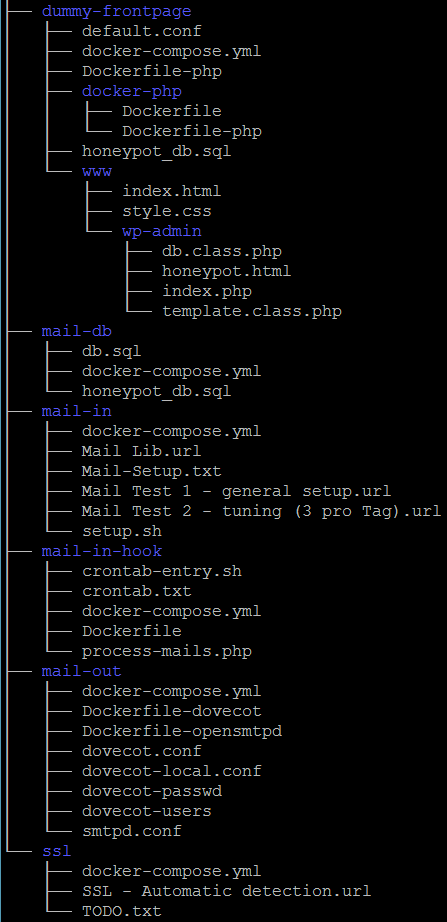
\includegraphics[scale=0.9]{hostTree.png}
	 	\caption{Hostsystem - Ordnerstruktur}
		\label{fig:HostsystemOrdnerstruktur}
	\end{figure}	
	
	\subsection{Eingangsserver}\label{sec:UmsetzungEingangsserver}
		Der Mail-Eingangserver besteht aus den Compenenten Docker-Mailserver-Image und dem Datenbank Script. Des weiteren wird noch ein SSL-Zertifikat benötigt welches die Authentizität der Mails Sicherstellt und eine SQL-Datenbank um die Mails zu persistieren. Im folgenden Abschnitt wird die konfiguration dieser Docker-\nameref{itm:Container} vorgenommen.
		\subsubsection{Docker Konfiguration}\label{Mail-In-Container}
			%referenz zum docker image und konfig code
			Es wird ein Docker-Image-Mailserver verwendet, dieser wird als Docker-Image eingebunden und konfiguriert. Um Mails empfangen und per IMAP über einen Mail Client beziehen zu können werden die folgende Ports benötigt:
		\begin{itemize}
			\item
				25 für TLS SMTP
			\item
				143 TLS IMAP
			\item
				587 TLS default mail submission port
			\item
				993 SSL IMAP
			Spam soll nicht gefiltert oder geblockt werden, daher werden Module wie Spamassassin, Clamav, Fail2ban, Postgrey und Spoof-Protection deaktiviert.
		\end{itemize}
			
		\subsubsection{SSL Konfiguration}\label{SSl-Container}
			%referenz zum ssl docker code
			Das beziehen der SSL-Zertifikate erfolg über den SSL-Docker-Container, dieser wurde vorkonfiguriert bezogen und wird dann angepasst um automatisch die Zertifikate auszustellen und zu prüfen.

		\subsubsection{Datenbank Container}\label{DB-Container}
%referenz zu DB-Container code
			Die Datenbank in der die Mails und auch die Fake-Mail-Aliases persistiert werden wird über ein Docker-Image eingebunden es handelt sich hierbei um eine mySQl Datenbank, um alle 30 Minuten die Mails in die Datenbank zu speichern wird hier ein PHP-Script per Cronjob aufgerufen. Zur Verwaltung der Datenbank wird PHPMyAdmin verwendet, hierfür muss noch der Port 80 benötigt welcher im Docker-\nameref{itm:Container} konfiguriert wird.

		\subsubsection{Datenbank PHP-Script}\label{DB-Hook-Container}
			Im Container für die Datenbank werden automatisch per PHP-Script die eingegangenen Mails gespeichert, hierfür werden die neun Emails über IMAP abgerufen und in die Datenbank gespeichert.

	\subsection{OpenRelay}\label{sec:UmsetzungOpenRelay} %Mario
		Um Spammer einen vermeintliches \nameref{itm:OpenRelay} für die Spamverteilung anzubieten, wird ein Mailserver konfiguriert, der von Mails von allen Adressen akzeptiert und wirkt als würde er diese weiterleiten.
		
		\subsubsection{OpenSMTPD}\label{OpenRelayOpenSMTPD}
			Da die Konfiguration des \textsf{OpenSmtpd} kompakt und einfach ist, wird mit diesem der \nameref{itm:OpenRelay} in einem Docker-\nameref{itm:Container} eingerichtet.
			
			Die Ports die nach außen im Netz verfügbar sind, werden dabei im Konfigurationsfile des Docker-\nameref{itm:Container} definiert. Darin werden außerdem die Speicherbereiche des \nameref{itm:Container}s mit den auf dem Host dafür vorgesehenen Speicher verlinkt und beim Start der VM gemounted. In diesem Speicherbereich auf dem Hostsystem werden auch die Konfigurationsdateien für den \textsf{OpenSmtpd} abgelegt. Darin ist die Weiterleitung für alle eingehenden Adressen an alle ausgehenden definiert. Darüber hinaus werden sämtliche Spamvorrichtungen deaktiviert, um für den Versand von sämtlichen Mails als Verteiler zu dienen.
			
			In Kombination mit einem Docker-\nameref{itm:Container} werden die Konfigurationen teils etwas anders umgesetzt. Bzw. wird die Kommunikation zwischen Mailserver Dienst im \nameref{itm:Container} und der \nameref{itm:Container} Konfiguration zum Host anders umgesetzt, als in den meisten Tutorials. Dies hat zur Folge das die Konfiguration eines \textsf{OpenSmtpd} innerhalb des Docker-\nameref{itm:Container} diverse Schwierigkeiten und Tücken mit sich bringt. 
			Nach zahlreichen Konfigurationsversuchen, die nicht zum gewünschten Erfolg geführt haben, wurde deshalb beschlossen das \nameref{itm:OpenRelay} auf eine andere Weise zu konfigurieren. Um innerhalb des Projektzeitraums noch den gewünschten Erfolg erzielen zu können.
			
		\subsubsection{Dovecot}\label{OpenRelayDovecot}
			Der gescheiterte Versuch den \nameref{itm:OpenRelay} mit einem \textsf{OpenSmtpd} eigenständig in einem Docker-\nameref{itm:Container} zu implementierten, wurde nun durch eine Konfiguration mit \nameref{sec:Dovecot} ergänzt.
			
			Dabei dient der \textsf{OpenSmtpd} als \nameref{itm:OpenRelay} der Mails von allen Absendeadressen an alle Zieladressen weiterleitet. Allerding werden diese nicht nach außen ins Internet weitergeleitet, sondern an den \nameref{sec:Dovecot} Service. Dieser dient als zusätzlicher SMTP-Knoten, an den der \textsf{OpenSmtpd} seine ausgehenden Mails weiterleitet. Der \nameref{sec:Dovecot} wird so konfiguriert, dass dieser keine Mails weiterleitet, sonder diese nur speichert. Somit versiegen die Mails die vom \textsf{OpenSmtpd} weitergeleitet werden. Trotzdem wirkt der \textsf{OpenSmtpd} als \nameref{itm:OpenRelay}, weil er weiter leitet und keine negative Rückmeldung an den Absender gibt.
			
			Die Komplikationen bei der Konfiguration des \nameref{itm:OpenRelay} haben dazu geführt, dass dieser erst zum Ende des Projektzeitraums publiziert werden kann. Somit werden sich die Erkenntnisse daraus voraussichtlich erst im Anschluss an dieses Projekt ergeben.


	\subsection{Adressen verbreiten}\label{sec:UmsetzungAdressenverbreiten}
		Um den Empfang von Spam sicher zu stellen, werden verschiedene Email-Adressen bei Diensten registriert und es wird auf die links in eingehenden E-Mails reagiert, bzw. geklickt. Dadurch sollten diese E-Mail-Adressen wirken als werden sie genutzt und somit für Spam Empfang sorgen. Im nachfolgenden wird beschrieben wie die umgesetzt wird.

		\subsubsection{Registrierung bei Diensten}\label{AdressenVerbreitenRegistrierenDiensten}
		Zuerst wurden bei Diversen Diensten wie z.b. Facebook, Twitter, Parship usw. Konten mit Fake-Daten und Catch-All-Mail-Adressen registriert, danach wurde geschaut ob durch die Dienste und/oder Diensten von dritten noch mehr Fake-Mails registriert werden können. im Anschluss wurde versucht die Konten bei Diensten als aktiv wirken zu lassen durch z.b. ändern von Profildaten und anklicken der Links in erhaltenen Mails. Da im Mai 2019 auf den E-Mail-Adressen der Fachhochschule Ravensburg-Weingarten Spammails eingingen wurden auch dort Catch-All-Mail-Adressen registriert um direkt diese Spammer zum senden weiteren Spams anzuregen.
		
		\subsubsection{Reaktion auf Spam}\label{AdressenVerbreitenReaktionSpam}
		Auf die eingehenden Spammails wird von Hand reagiert, d.h. links werden angeklickt und die jeweilig verlinkten Seiten angeschaut. Vor allem wird geschaut ob sich evtl. noch mehr Mails bei den verlinkten Diensten registrieren lassen und ob man durch eine Anmeldung mit Fake-Daten evtl. den Erhalt von mehr Spam beschleunigen kann.
	
	\subsection{Website}\label{sec:UmsetzungWebsite}
		Um auch durch \nameref{itm:crawler} auf Spammerlisten zu landen wird eine statische Webseite angelegt, hierfür wird ein Docker-Webserver-Container aufgesetzt und eine HTML Seite angezeigt.

		\subsubsection{Webservice}\label{WebsiteWebservice}
			Für den Container wird ein nginx:alpine Docker-Image geladen und konfiguriert so das beim Aufruf einer URL eine statische Seite angezeigt wird die statische Einträge mit E-Mail-Adressen enthält, hierfür wird der Port 80/TCP benötigt.
			
		\subsubsection{HTML-Seite}\label{WebsiteHTML-Seite}
			Um den Erhalt von Spam Nachrichten zu beschleunigen wird eine \nameref{itm:HTML}-Webseite mit E-Mail Einträgen angelegt, diese Webseite ist statisch und erfüllt nur den Zweck von \nameref{itm:crawler}n gefunden zu werden, welche diese dann an Spammer weiterleiten könnten.

\newpage

	
\section{Fazit}\label{sec:Fazit}
%	Fazit knüpft bei Einleitung an (bzw. Literaturüberblick - den haben wir nicht)
%	"Wir" ist hier erlaubt
%	TODO

\newpage


% Quotes
\bibliography{zitate}
\bibliographystyle{plain}
\addcontentsline{toc}{section}{Literatur}
\newpage


% Image listing
\listoffigures
\addcontentsline{toc}{section}{Abbildungsverzeichnis}
\newpage


% Listings (code examples, ...)
% Enable bash style
\definecolor{dkgreen}{rgb}{0,0.6,0}
\definecolor{mauve}{RGB}{224, 176, 255}
\lstset{
  language=bash,
  keywordstyle=\color{blue},
  commentstyle=\color{dkgreen},
  stringstyle=\color{mauve},
  numbers=left,
  basicstyle=\scriptsize\ttfamily,
  showspaces=false,
  frame=shadowbox,
  xleftmargin=0.5cm,
  escapeinside={(*@}{@*)},
  morecomment={[l]\#\ }
}
\addcontentsline{toc}{section}{Listings}
\lstlistoflistings
\begin{lstlisting}[caption={Maileingangsserver}]
mail-in:
  container_name: mail-in
  ports:
    - "25:25/tcp"
    - "143:143/tcp"
    - "587:587/tcp"
    - "993:993/tcp"
  hostname: mail
  domainname: example.com
  environment:
    # One dir for docker backups
    - ONE_DIR=1
    
    # Debug
    - DMS_DEBUG=1
    
    # Disable modules
    - ENABLE_SPAMASSASSIN=0
    - ENABLE_CLAMAV=0
    - ENABLE_FAIL2BAN=0
    - ENABLE_POSTGREY=0
    - SPOOF_PROTECTION=0
    
    # Embed ssl manually
    - SSL_TYPE=manual
    - SSL_CERT_PATH=/etc/manual-ssl/signed.crt
    - SSL_KEY_PATH=/etc/manual-ssl/domain.key
    
    # Set the post master
    - POSTMASTER_ADDRESS=postmaster@example.com
  image: tvial/docker-mailserver:latest
  volumes:
    - ../DATA/mail-in/data:/var/mail
    - ../DATA/mail-in/state:/var/mail-state
    - ../DATA/mail-in/config:/tmp/docker-mailserver
    - ../DATA/mail-in/logs:/var/log/mail
    # Mount the ssl for this service manually
    - ../DATA/ssl/mail.example.com/production:/etc/manual-ssl
  cap_add:
    - NET_ADMIN
    - SYS_PTRACE
  tty: true
  stdin_open: true
  restart: always
	\end{lstlisting}
	\begin{lstlisting}[caption=SSL-Container]
ssl:
  container_name: ssl
  ports:
    - "80:80/tcp"
    - "443:443/tcp"
  environment:
    DOMAINS: 'mail.example.com'
    STAGE: 'production'
    SERVER_NAMES_HASH_BUCKET_SIZE: 64
    CLIENT_MAX_BODY_SIZE: 0
  image: steveltn/https-portal:1.6.1
  volumes:
    - ../DATA/ssl:/var/lib/https-portal
    # Enables a docker lookup of services for
    # them to configure https themselves
    - /var/run/docker.sock:/var/run/docker.sock:ro
  tty: true
  stdin_open: true
  restart: always
	\end{lstlisting}
	\begin{lstlisting}[caption=DB-Container]
db:
  container_name: mail-db
  environment:
    MYSQL_ROOT_PASSWORD: YOUR_PASSWORD
    MYSQL_DATABASE: mail
  image: mysql:5.7
  volumes:
    - ../DATA/mail-db/mysql:/var/lib/mysql
  tty: true
  stdin_open: true
  restart: always

phpmyadmin:
  container_name: mail-db_phpmyadmin
  ports:
    - "14080:80/tcp"
  image: phpmyadmin/phpmyadmin
  links:
    - db
  tty: true
  stdin_open: true
  restart: always
	\end{lstlisting}
\newpage


% Additional stuff
\section*{Anhang}\label{Anhang}
\addcontentsline{toc}{section}{Anhang}
\newpage


% Plagiarism declaration
\begin{newpage}
\vspace*{\fill}
\section*{Eidesstattliche Erklärung}\label{sec:Eidesstattliche Erklärung}
\addcontentsline{toc}{section}{Eidesstattliche Erklärung}
	Hiermit versichere ich, die vorliegende Arbeit selbstständig und unter ausschlie{\ss}licher Verwendung der angegebenen Literatur und Hilfsmittel erstellt zu haben. Die Arbeit wurde bisher, in gleicher oder ähnlicher Form, keiner anderen Prüfungsbehörde vorgelegt und auch nicht veröffentlicht.\\

\vspace{3cm}
\begin{tabular*}{\textwidth}{c@{\extracolsep\fill}cc}
\cline{1-1}
\cline{3-3}
\\
\ \ \ \ \ \ \ \ \ Unterschrift\ \ \ \ \ \ \ \ \ \ & & \ \ \ \ \ \ \ \ \ Ort, Datum\ \ \ \ \ \ \ \ \ \\
\end{tabular*}
\end{newpage}

\end{document}
